% supplement.tex: standalone Supplementary Material.
% Compiles to output/supplement/supplement.pdf via
% scripts/paper/build_supplement.jl.
%
% Figures S1--S3 describe the matching-function data-generating process. Figure S4
% compares assessment and access across matching composition. Figures S5--S7
% reproduce the structural analyses with two alternative network measures.
% Caption values come from retained-data reporting fragments.

\documentclass[11pt]{article}
\usepackage[letterpaper,margin=1in]{geometry}
\usepackage{amsmath,amssymb,graphicx}
\usepackage[font=small,labelfont=bf]{caption}
\graphicspath{{../output/supplement/figures/}}

% Supplement figure numbering: S1, S2, ...
\renewcommand{\thefigure}{S\arabic{figure}}

% Minimal key/value store so generated display conventions appear as \pv{key}
% rather than literals (mirrors the results pipeline's \pvDefine/\pv contract).
\makeatletter
\newcommand{\pvDefine}[2]{\expandafter\def\csname pv@#1\endcsname{#2}}
\newcommand{\pv}[1]{%
  \expandafter\ifx\csname pv@#1\endcsname\relax
    \GenericError{}{Supplement: undefined \string\pv{#1}}{}{}%
  \else\csname pv@#1\endcsname\fi}
\makeatother
% supp_figmeta.tex: generated by scripts/paper/supp_figures.jl. Do not edit by hand.
% DGP data analysis commit: e3f041b8a284bda48bf98907d9f7b42521987b07
% Structural data analysis commit: e3f041b8a284bda48bf98907d9f7b42521987b07
% Rendering commit: de4d915ddec550d37df54fca4da1f5ba3e0af5c1
% Source fingerprint: e7f85ed64c339dd02722d14ab76531f911850b09027b321adc51bcdc340e260c
% Source SHA256: Manifest.toml f46bb7b8de59a31243453fd46f7d8f56323e3a5c654c05f6372c70233786d00d
% Source SHA256: Project.toml f1a16964dc901c82ab1ce764d7b64e04510d55237b1a261f06a204300a694649
% Source SHA256: scripts/figure_style.jl 3cd09ee32da2a43dabc265a11917403f0b84b0c7bd157c3263d27c3d115d089f
% Source SHA256: scripts/monte_carlo.jl dd2fc88b57e8b8b5315fb210eee1268eb5eea4e4a2bf28dae0670d4c0730ef03
% Source SHA256: scripts/paper/supp_figures.jl 138f6f2677c1083d8e4b9ac7e5b78a2a34da93c486f9f4340e2cbc9d65c727ca
% Source SHA256: scripts/reporting_provenance.jl a804a4bf0895e0880d78a5630f5ecfbaa903d31fdb3c8ba7e07fb377abc285b5
% Exploratory DGP artifact: false
% Exploratory rendering: false
% Display conventions used to render output/supplement/figures/, quoted in captions via \pv keys.
\pvDefine{suppRollWin}{5}
\pvDefine{suppMeasInterval}{20}
\pvDefine{suppAxisStart}{30}
\pvDefine{suppRegimeN}{80}
\pvDefine{suppOatN}{26}
\pvDefine{suppDgpSeeds}{50}
\pvDefine{suppDgpN}{1000}
\pvDefine{suppDgpHeatmapN}{100}
\pvDefine{suppDgpHeatmapSeed}{1}
\pvDefine{suppDgpDelta}{0.5}
\pvDefine{suppDgpSpectrumComponents}{25}
\pvDefine{suppDgpRankEnergyPercent}{90}

% paper_values.tex: generated by scripts/assessment_access/paper_values.jl
% Generated: 2026-09-14 13:16
% Data analysis commit: 99024c548648adbf353258ca3679614f7642722c
% Retained analysis source clean: true
% Sweep commit: eb2f77168aa31c4b113cd77c9d3caf92de5b08fa
% Manifest: ce48b8c9cbc9d3fa217f2b603b6124f11f1abd71869d6b600bffe0f7ad45c011
% Supplement manifest: 1b9dd482ca66b033b6a46e561d6e0c4fc7d61598131e03557ec720792a146cd3
% Manuscript formatting commit: 79fd29611cc083f703ba36f36b371c473695cf20
% Manuscript formatting source clean: true
% Formatter SHA256: 00ae2c8f707c6af6da37007383ba6e151a62be7d4b0eeb10546165e33d135d27
% Figure data SHA256: 2a7a5cdf14ea409985444fa59ee85b050ef63f6cf7dd521149168c2f32e6e124
% Trajectory data SHA256: 3d73d3dff3dcaad49e44a1c5bc1f9fe324419e5867015e08ea5c83af18a84c93
% Do not edit: all scientific values derive from retained data or metadata.
\pvDefine{aaRho}{0.5}
\pvDefine{aaDelta}{0.5}
\pvDefine{aaEta}{0.02}
\pvDefine{aaEtas}{0,0.001,0.01,0.02,0.03}
\pvDefine{aaEtaCount}{5}
\pvDefine{aaAccessLossEtas}{0.01,0.02,0.03}
\pvDefine{aaEtaSmall}{0.001}
\pvDefine{aaEtaLower}{0.01}
\pvDefine{aaEtaUpper}{0.03}
\pvDefine{aaLateWidth}{20}
\pvDefine{aaLateStart}{481}
\pvDefine{aaHorizon}{500}
\pvDefine{aaN}{1{,}000}
\pvDefine{aaDegreeStart}{1}
\pvDefine{aaCentralityFirst}{20}
\pvDefine{aaCentralitySecond}{40}
\pvDefine{aaIntervalPercent}{95}
\pvDefine{aaBaselineSeeds}{50}
\pvDefine{aaOtherSeeds}{20}
\pvDefine{aaAccessOutputLoss}{0.242}
\pvDefine{aaAssessmentOutputLoss}{0.309}
\pvDefine{aaAssessmentAccessOutputDifference}{0.067}
\pvDefine{aaAssessmentAccessOutputLower}{0.048}
\pvDefine{aaAssessmentAccessOutputUpper}{0.086}
\pvDefine{aaFullOutPercent}{96.8}
\pvDefine{aaFullDegree}{17.727}
\pvDefine{aaAssessmentOutPercent}{97.1}
\pvDefine{aaAssessmentDegree}{15.523}
\pvDefine{aaAssessmentCentralityDifference}{+0.060}
\pvDefine{aaAssessmentCentralityLower}{0.051}
\pvDefine{aaAssessmentCentralityUpper}{0.069}
\pvDefine{aaAccessOutPercent}{82.0}
\pvDefine{aaAccessDegree}{25.611}
\pvDefine{aaAccessCentralityDifference}{-0.178}
\pvDefine{aaAccessCentralityLower}{-0.196}
\pvDefine{aaAccessCentralityUpper}{-0.161}
\pvDefine{aaAccessBrokerRank}{0.982}
\pvDefine{aaAccessPrincipalRank}{0.708}


\setlength{\parskip}{0.6\baselineskip}
\setlength{\parindent}{0pt}
\clubpenalty=10000
\widowpenalty=10000
\displaywidowpenalty=10000
\renewcommand{\topfraction}{0.85}
\renewcommand{\bottomfraction}{0.8}
\renewcommand{\textfraction}{0.1}
\renewcommand{\floatpagefraction}{0.85}
\setcounter{topnumber}{2}
\setcounter{bottomnumber}{2}
\setcounter{totalnumber}{4}

\begin{document}

\begin{center}
{\large\bfseries Supplementary Material}\\[2pt]
{\large Model Structure, Assessment and Access, and Network Measures}
\end{center}

Figure~\ref{fig:supp-type-geometry} illustrates the baseline type distribution. Figures~\ref{fig:supp-dgp-structure}--\ref{fig:supp-dgp-dimension} describe the match-value function under that distribution. Within each realization, principal types and the matching-function objects $c$, $A$, and $B$ are held fixed while $\rho$ and $\delta$ vary. The match-value figures show the conditional value $E[q_{ij}\mid x_i,x_j]=Q+f(x_i,x_j)$, without match noise. They therefore isolate the structure principals and the broker must learn rather than variation from one set of noisy outcomes.

Figure~\ref{fig:supp-assessment-access} compares the contributions of assessment and access across matching composition and turnover.

Figures~\ref{fig:supp-grid}--\ref{fig:supp-advantage} reproduce the main structural analyses using Burt's aggregate network constraint and effective size. Constraint summarizes the concentration of the broker's direct and indirect ties. Effective size discounts contacts that are connected to one another. Both are computed for the broker every \pv{suppMeasInterval} periods. A regime is one scientifically distinct parameter configuration; duplicate grid coordinates and inactive parameters do not create additional regimes.

\begin{figure}[htbp]
\centering
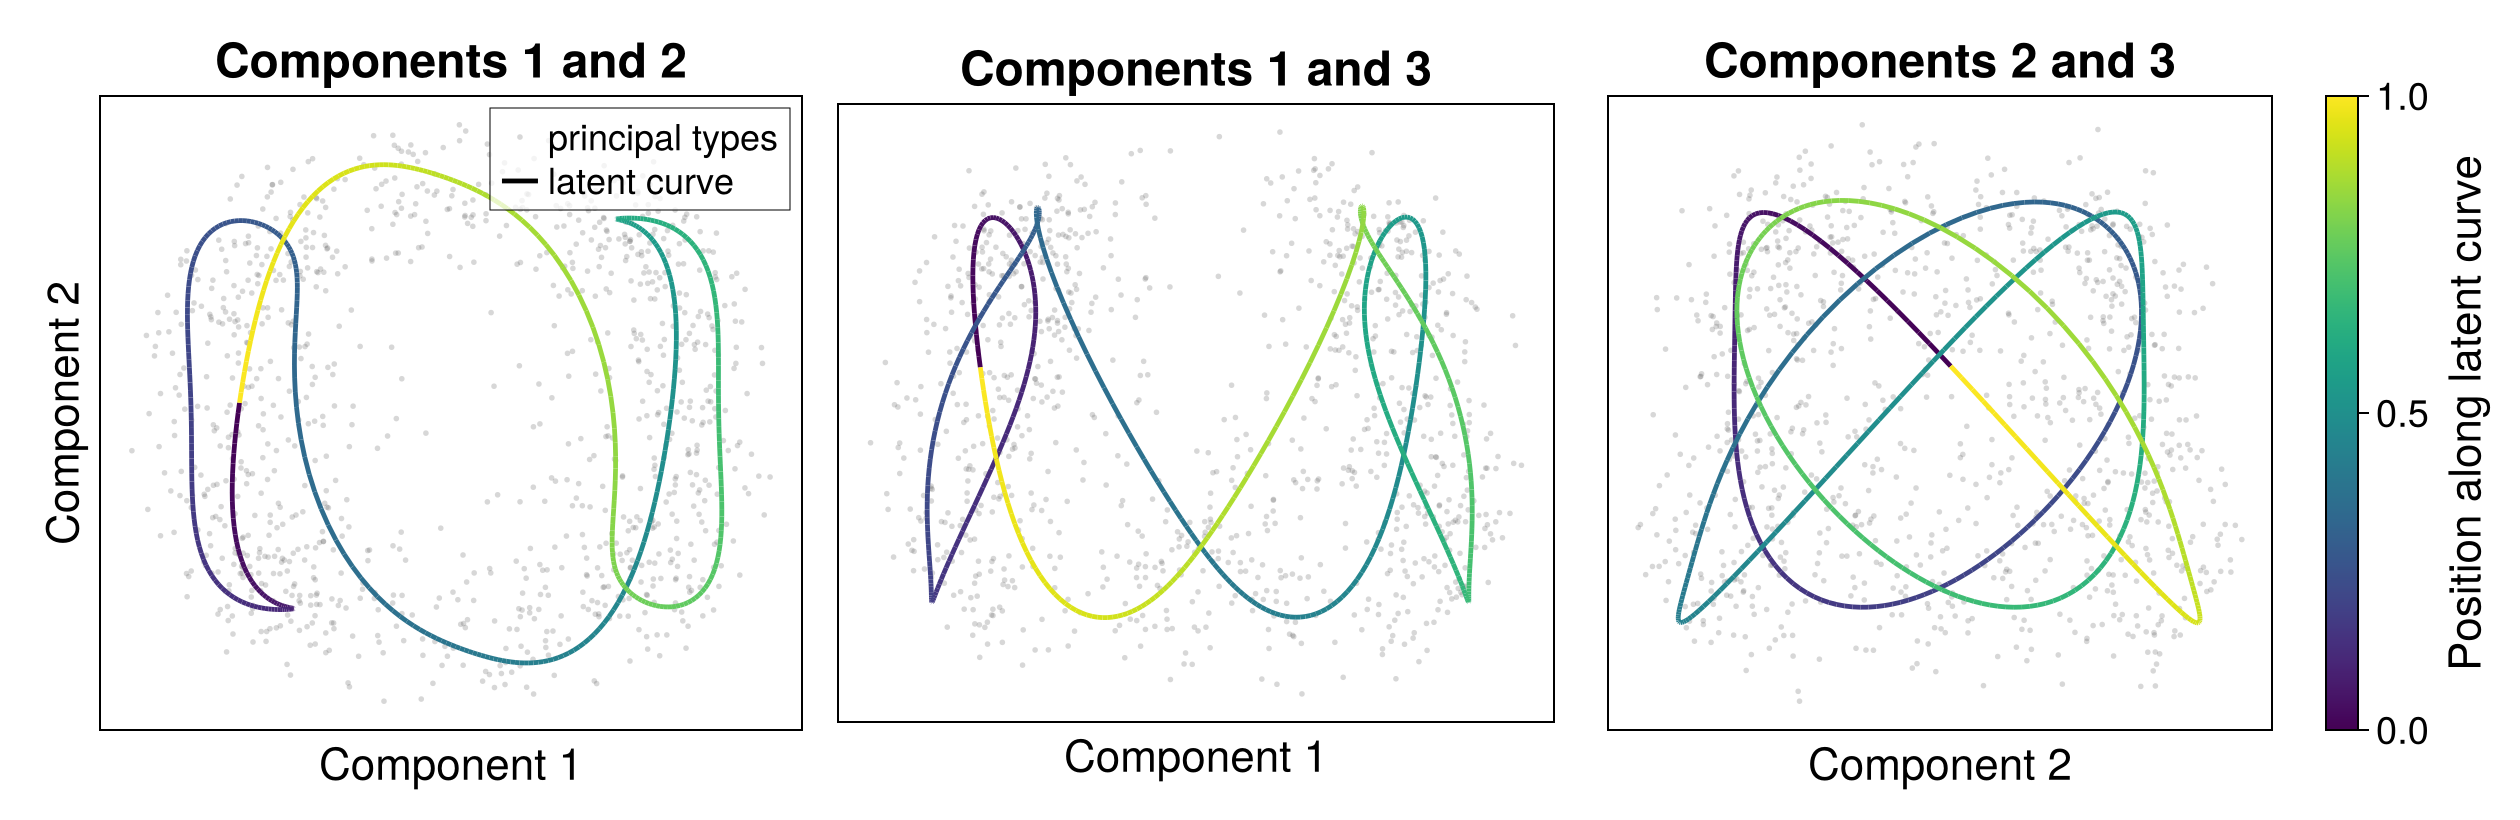
\includegraphics[width=\linewidth]{type_geometry.png}
\caption{\textbf{Principal types and their latent curve.} Three projections of all \pv{suppDgpN} baseline principal types in realization \pv{suppDgpHeatmapSeed}. Types are drawn around a smooth latent curve and projected to the unit sphere in eight-dimensional type space. A--C show pairs of the curve's first three principal components. Gray points are realized types; the colored line is the latent curve, with color indicating position along it. These projections are for visualization only; matching and learning use the full eight-dimensional types.}
\label{fig:supp-type-geometry}
\end{figure}

\begin{figure}[htbp]
\centering
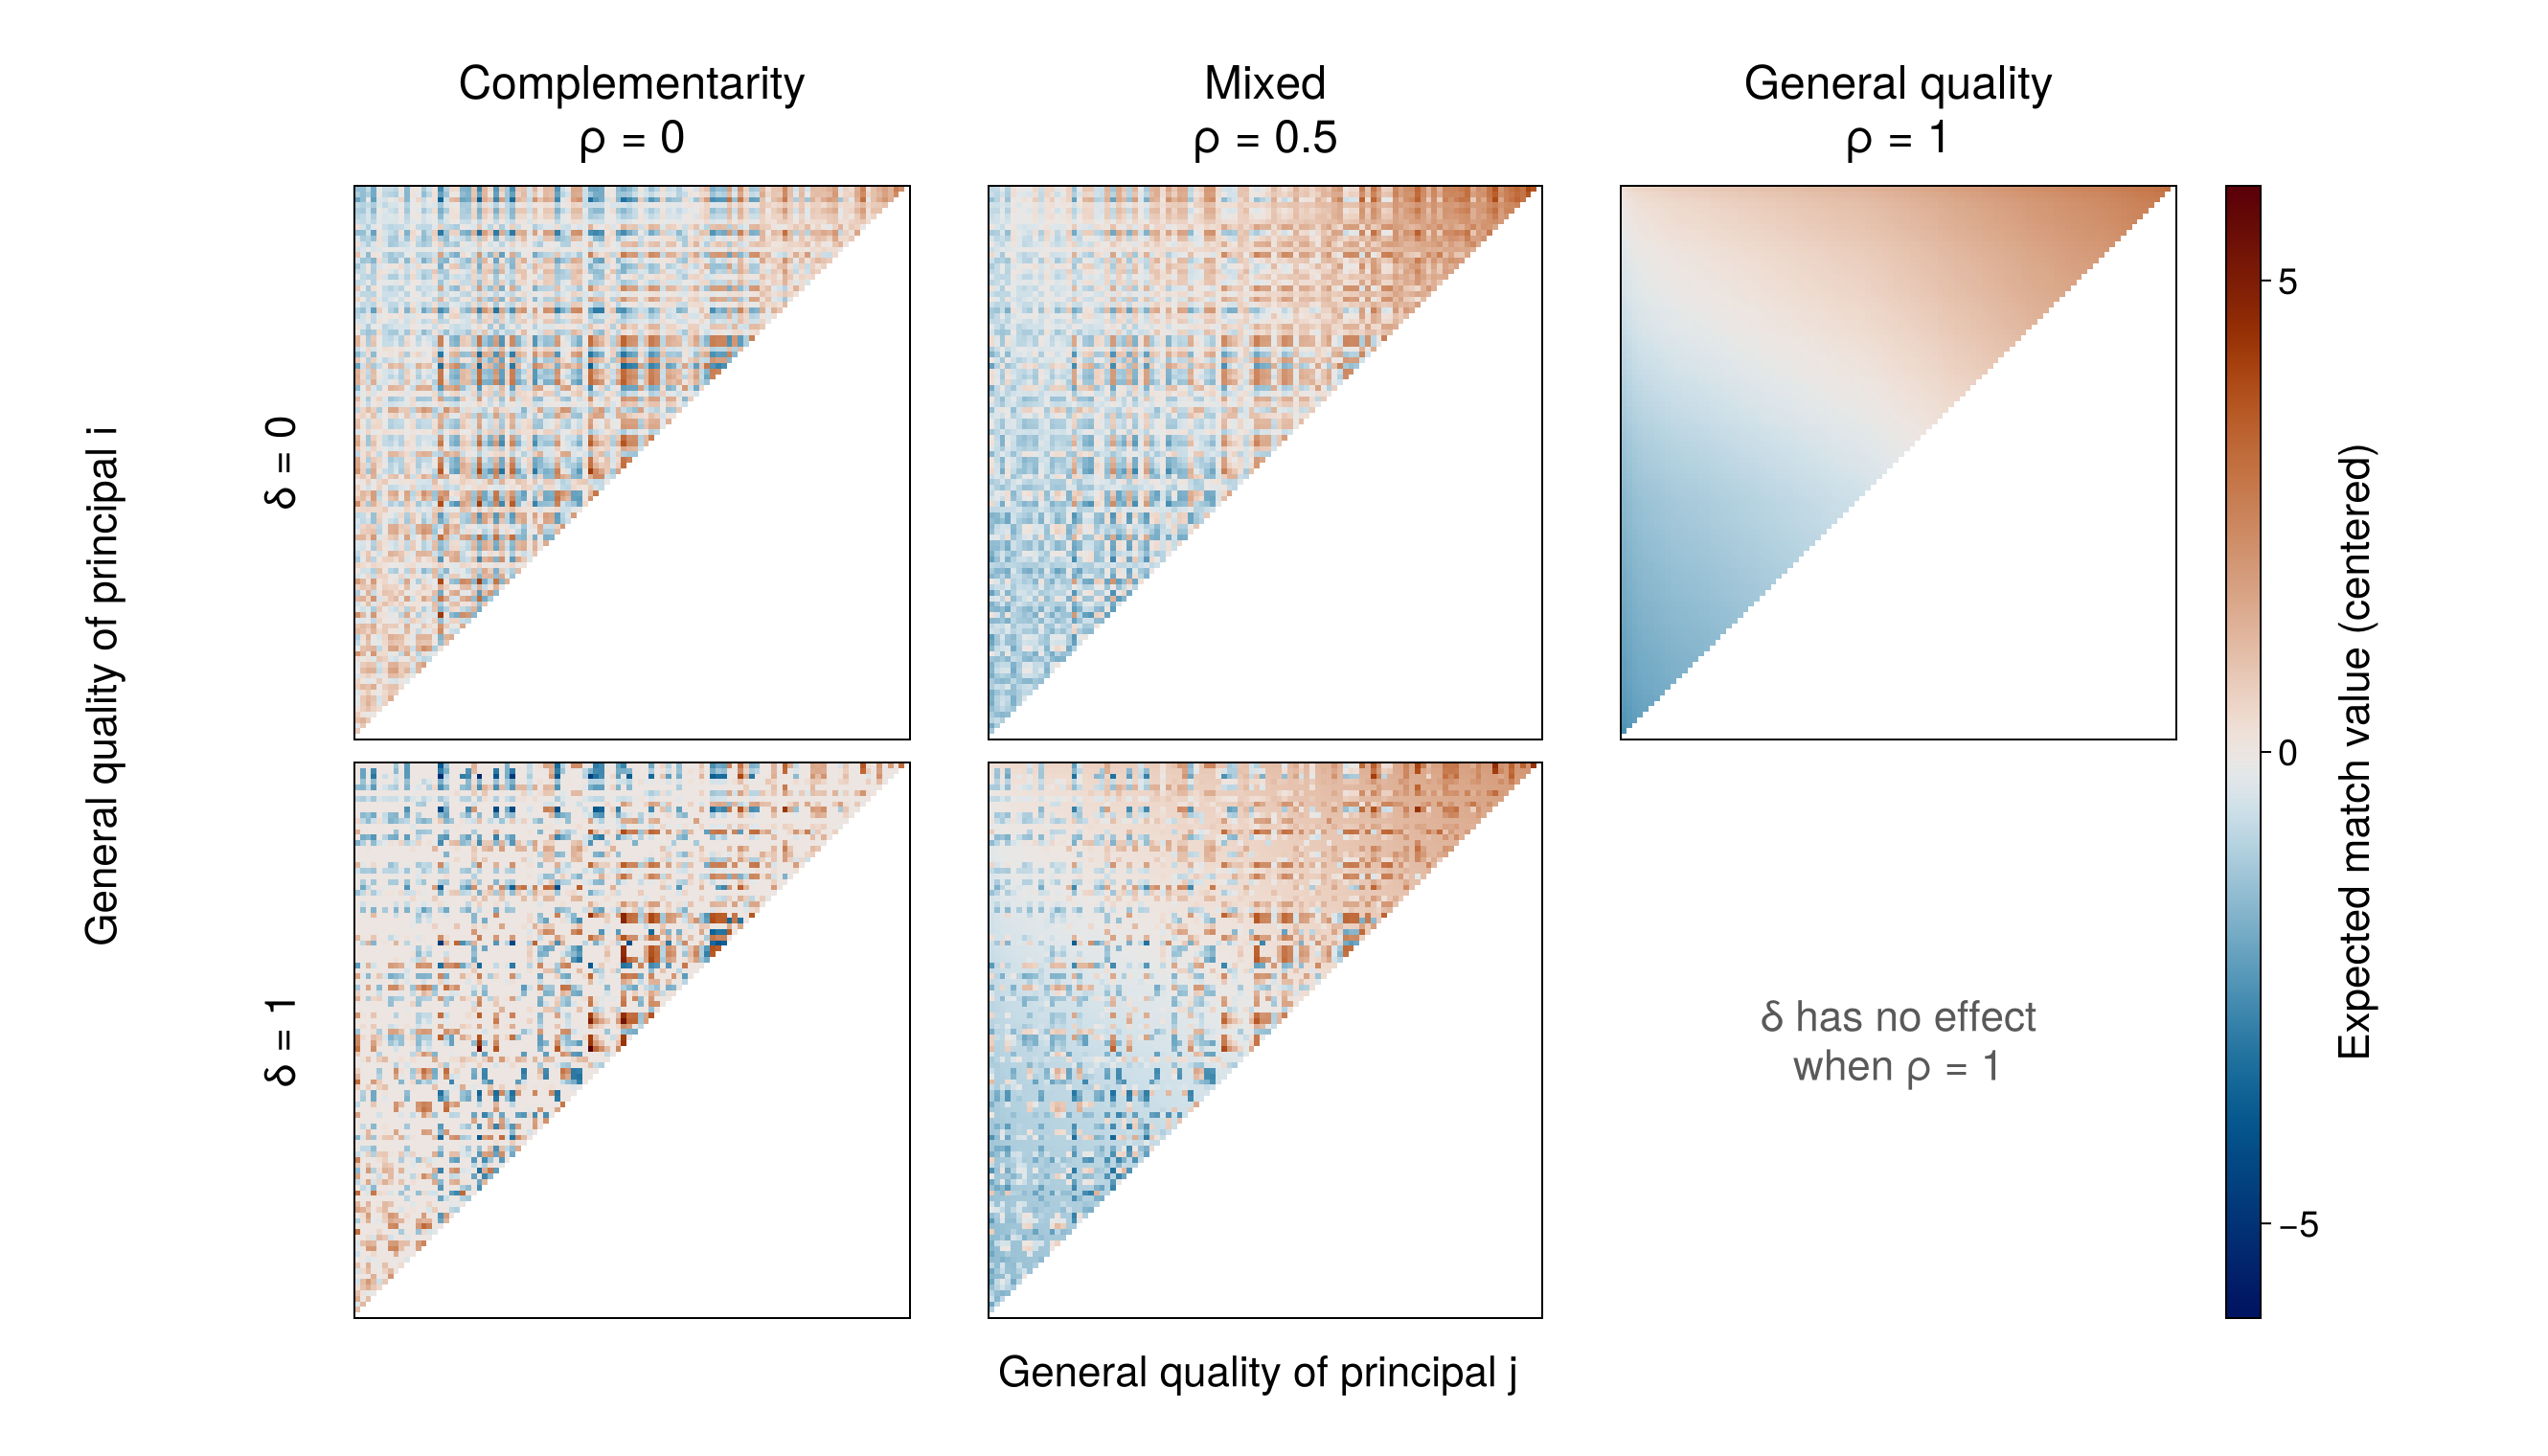
\includegraphics[width=\linewidth]{match_value_surfaces.png}
\caption{\textbf{Expected match output across pairs of principal types.} Centered conditional output for \pv{suppDgpHeatmapN} types selected at evenly spaced general-quality ranks from a $\pv{suppDgpN}$-principal realization (seed \pv{suppDgpHeatmapSeed}). Columns vary general-quality share $\rho$; rows compare low and high difficulty $\delta$. The pure-general-quality condition ($\rho=1$), where difficulty is inactive, is shown once. Types and matching-function objects $c$, $A$, and $B$ are fixed across panels. General quality increases from left to right and bottom to top. Only the upper triangle of each symmetric matrix is shown; self-matches on the diagonal are excluded. Colors use one shared scale. Matrices exclude match noise and subtract the grand mean. Normalization uses separate reference markets whose average within-market variance in predictable output across possible pairs equals one.}
\label{fig:supp-dgp-structure}
\end{figure}

\begin{figure}[htbp]
\centering
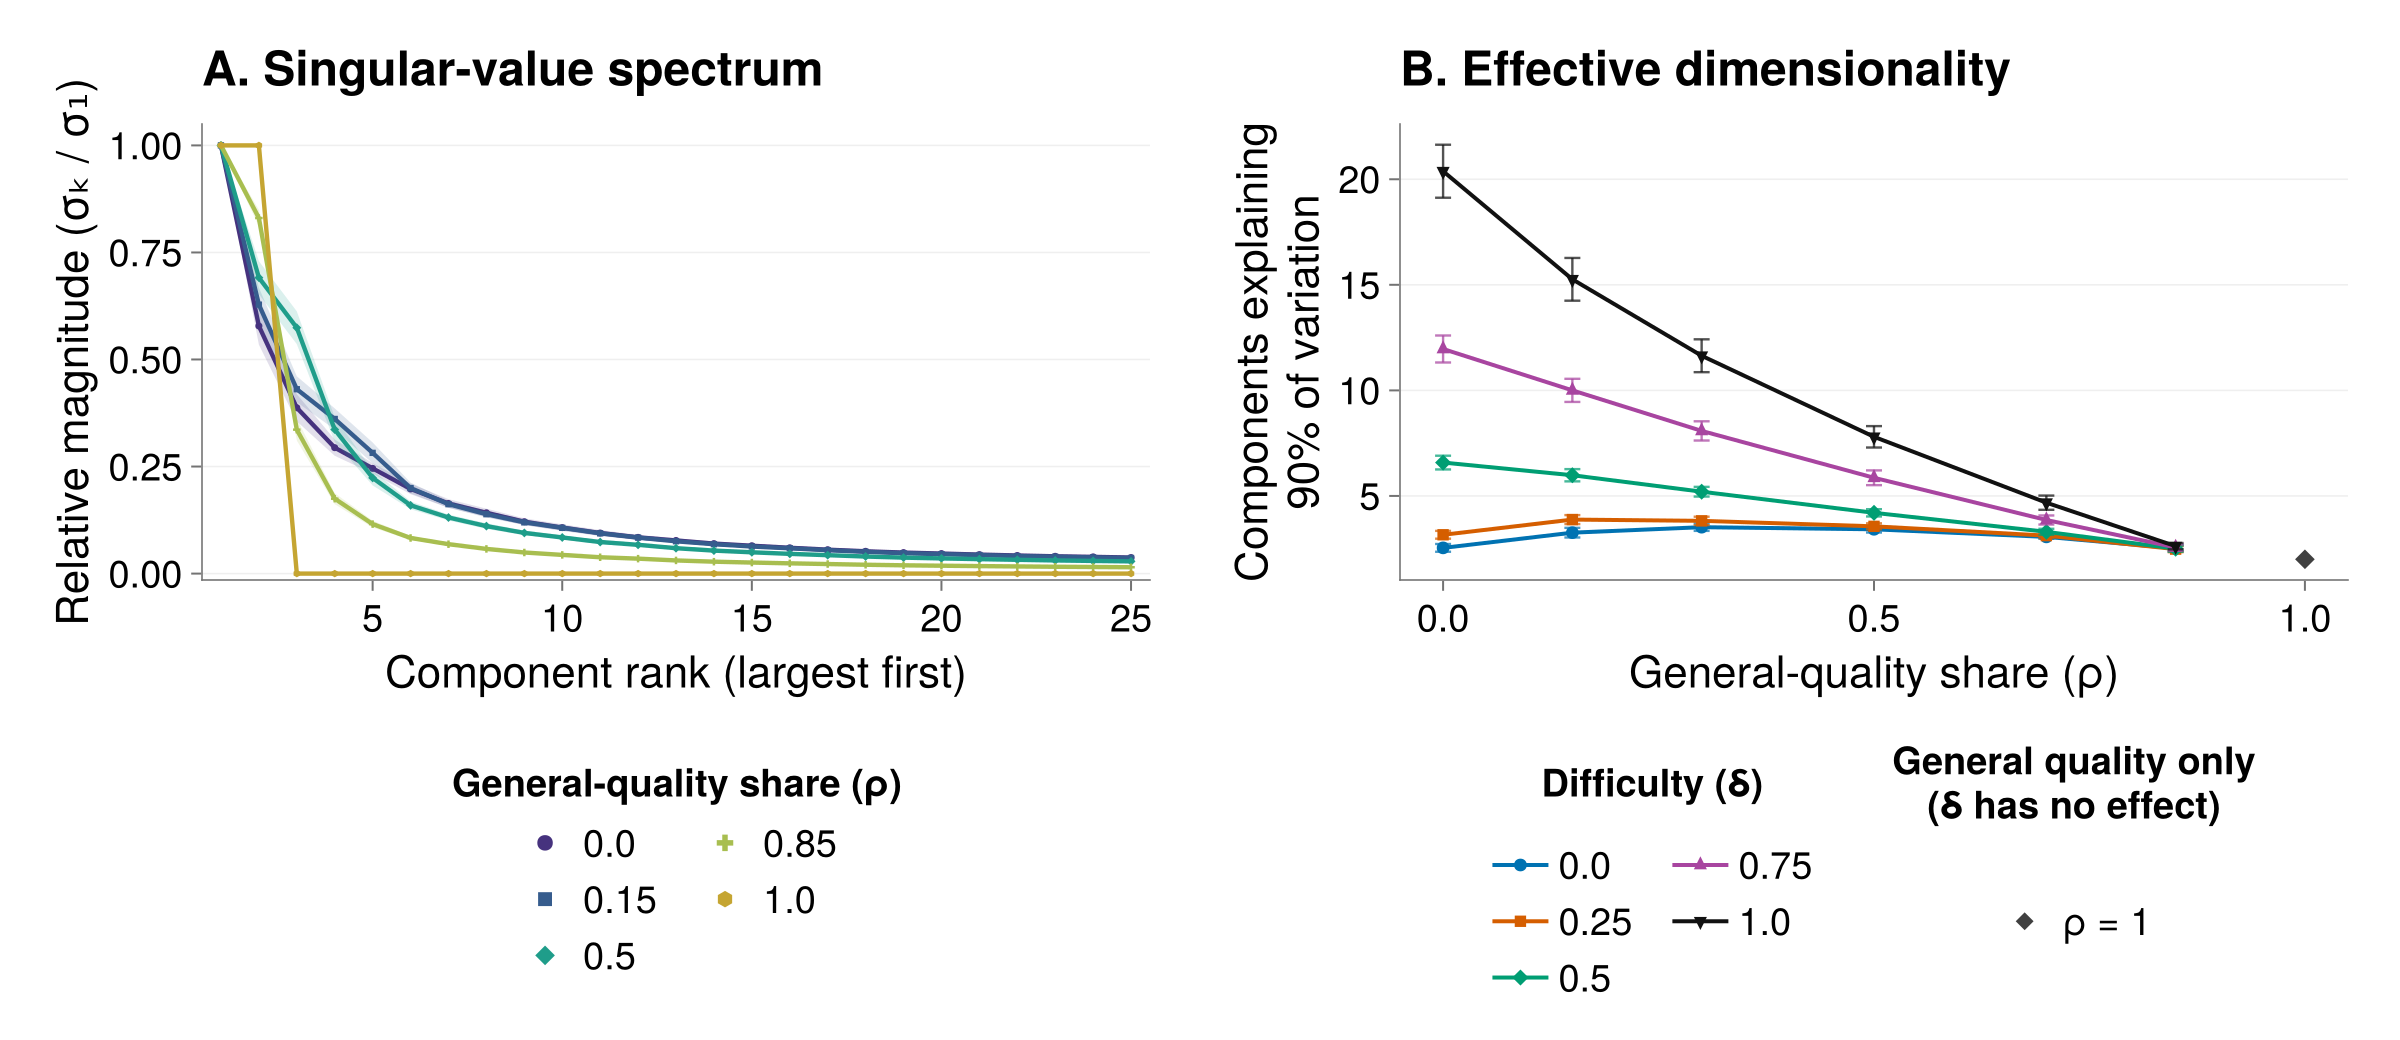
\includegraphics[width=\linewidth]{effective_dimensionality.png}
\caption{\textbf{Dimensionality of expected match output.} Summaries of the centered conditional-output matrix over \pv{suppDgpSeeds} independently generated sets of types and matching-function objects. A: the first \pv{suppDgpSpectrumComponents} singular values at $\delta=\pv{suppDgpDelta}$, each divided by the largest singular value within its realization. B: the minimum number of singular components accounting for \pv{suppDgpRankEnergyPercent}\% of the sum of squared singular values, calculated within each realization. Lines and markers are means across realizations; ribbons and whiskers are pointwise 95\% Monte Carlo intervals. Colors and symbols identify general-quality share $\rho$ in A and difficulty $\delta$ in B. General-quality share runs from pure complementarity (0) to pure general quality (1). In B, the $\rho=1$ boundary, where difficulty is inactive, is shown once and unconnected.}
\label{fig:supp-dgp-dimension}
\end{figure}

\begin{figure}[htbp]
\centering
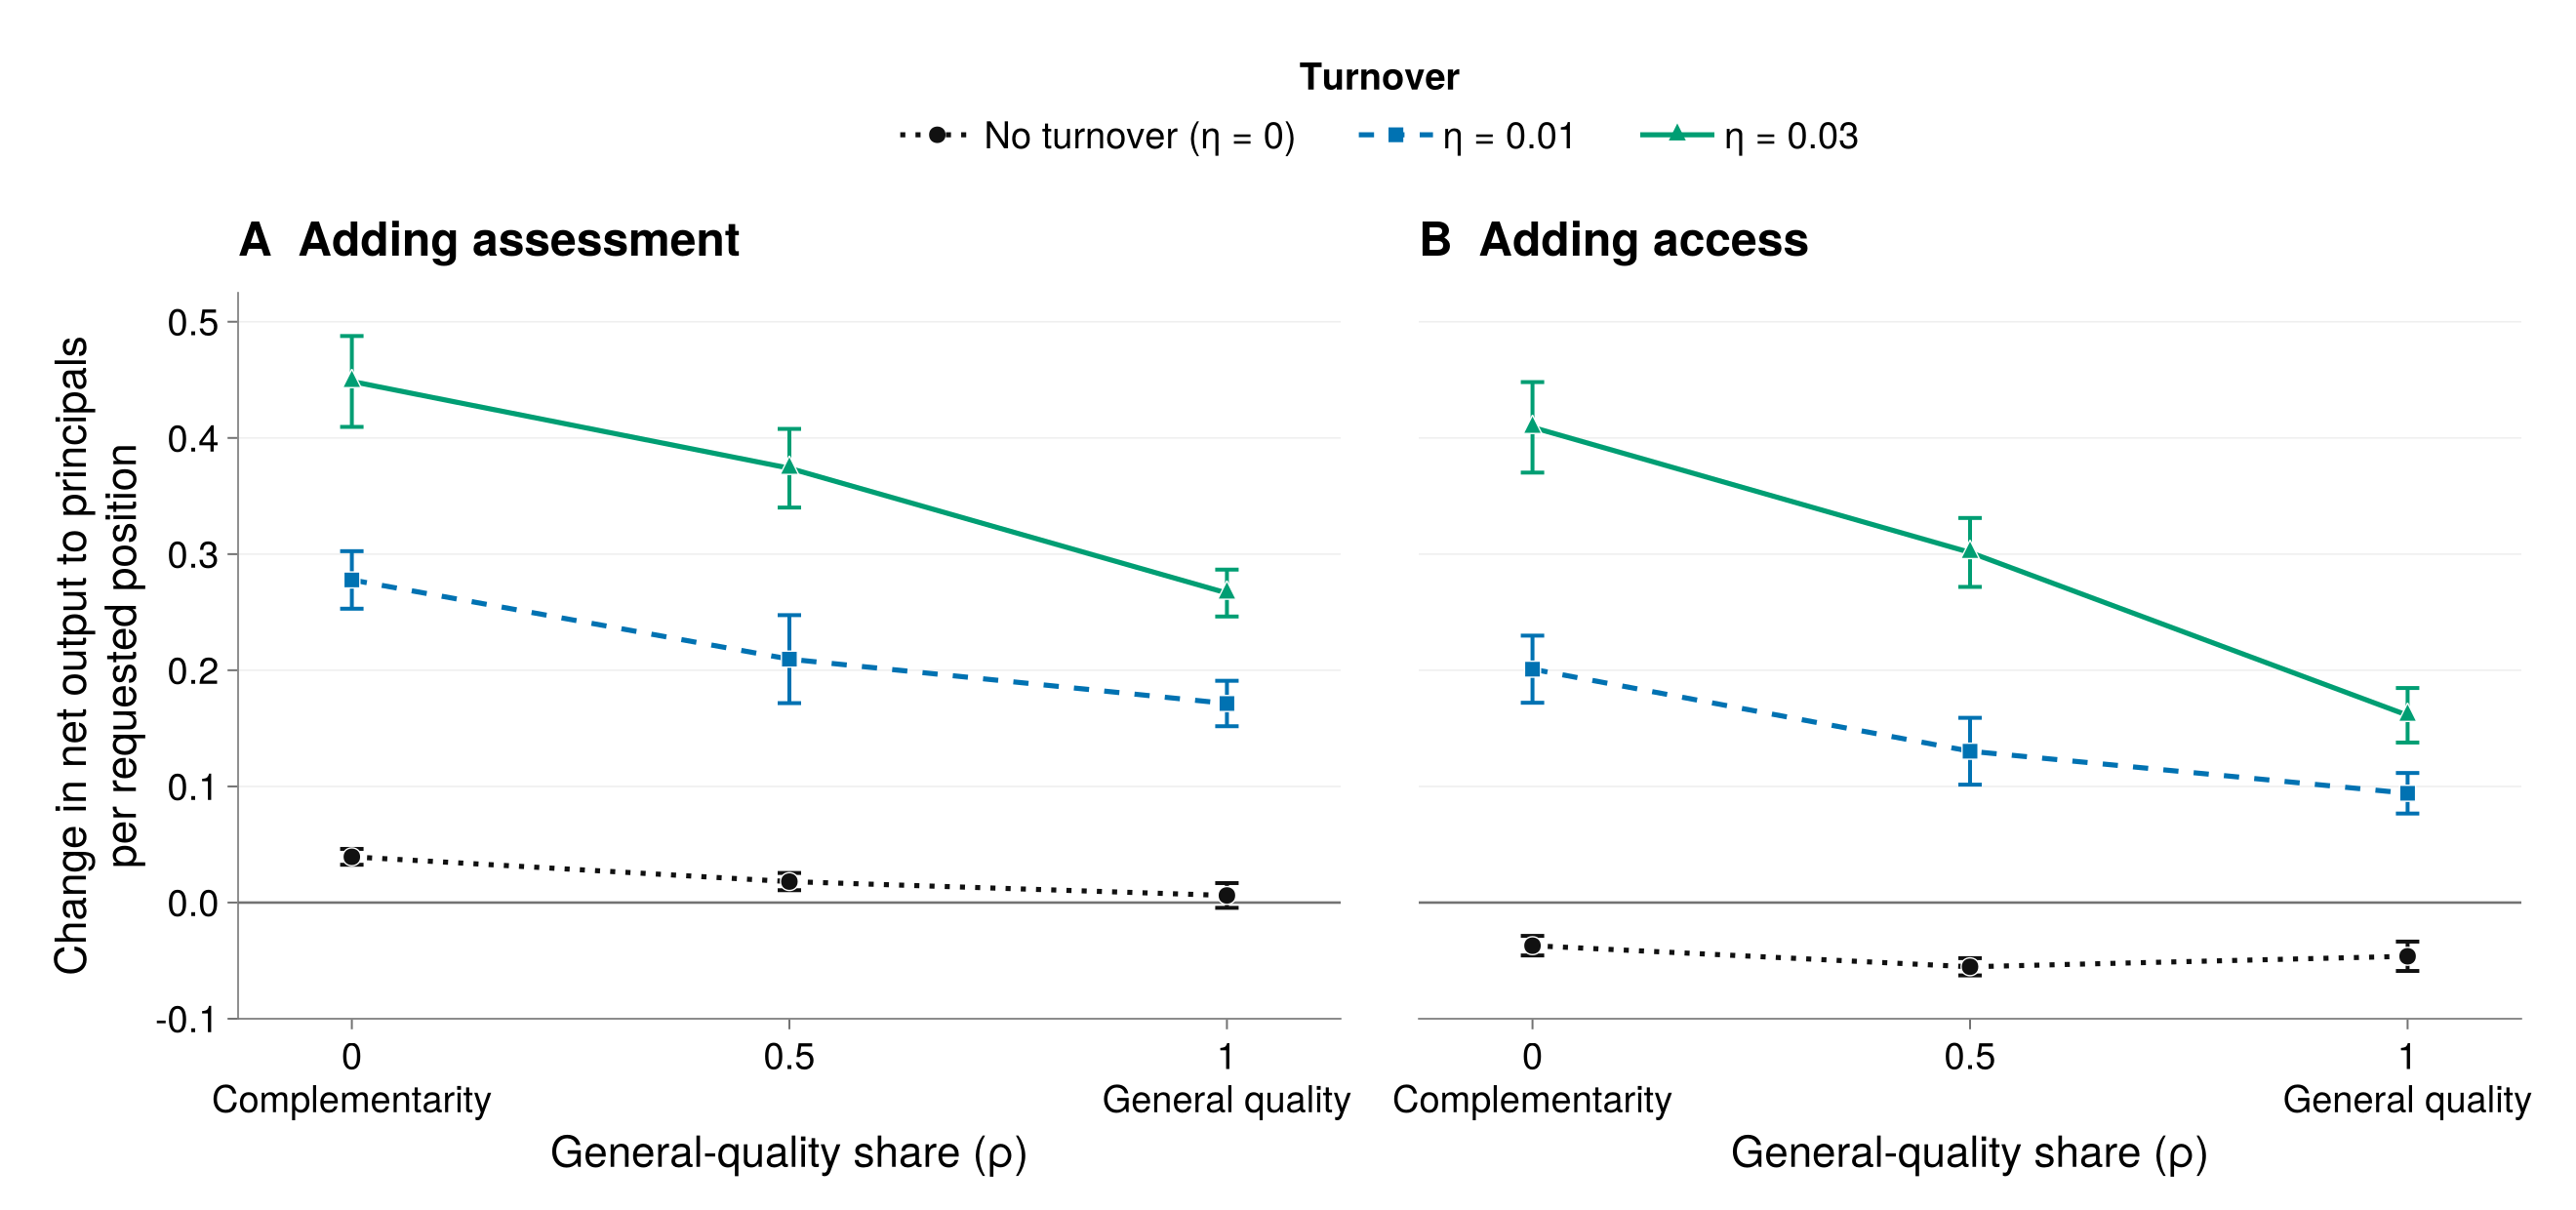
\includegraphics[width=\linewidth]{complementarity_contributions.png}
\caption{\textbf{Contributions of assessment and access across matching composition.} A: full service minus access-only in net output to principals per requested position. B: full service minus assessment-only. Broker models are defined in the main text. Net output deducts search costs and broker fees; unfilled positions remain in the denominator. Colors and symbols identify turnover $\eta$. Parameters other than general-quality share $\rho$ and turnover remain at baseline, including $\delta=\pv{aaDelta}$. Outcomes are averaged over $t=\pv{aaLateStart}$--$\pv{aaHorizon}$ within each seed. Within-seed differences are then averaged across \pv{aaOtherSeeds} seeds per condition. Bars are two-sided, pointwise \pv{aaIntervalPercent}\% Student-$t$ Monte Carlo intervals. Positive values indicate higher net output under full service. Panels share a vertical scale; lines connect tested conditions as visual guides.}
\label{fig:supp-assessment-access}
\end{figure}

\begin{figure}[htbp]
\centering
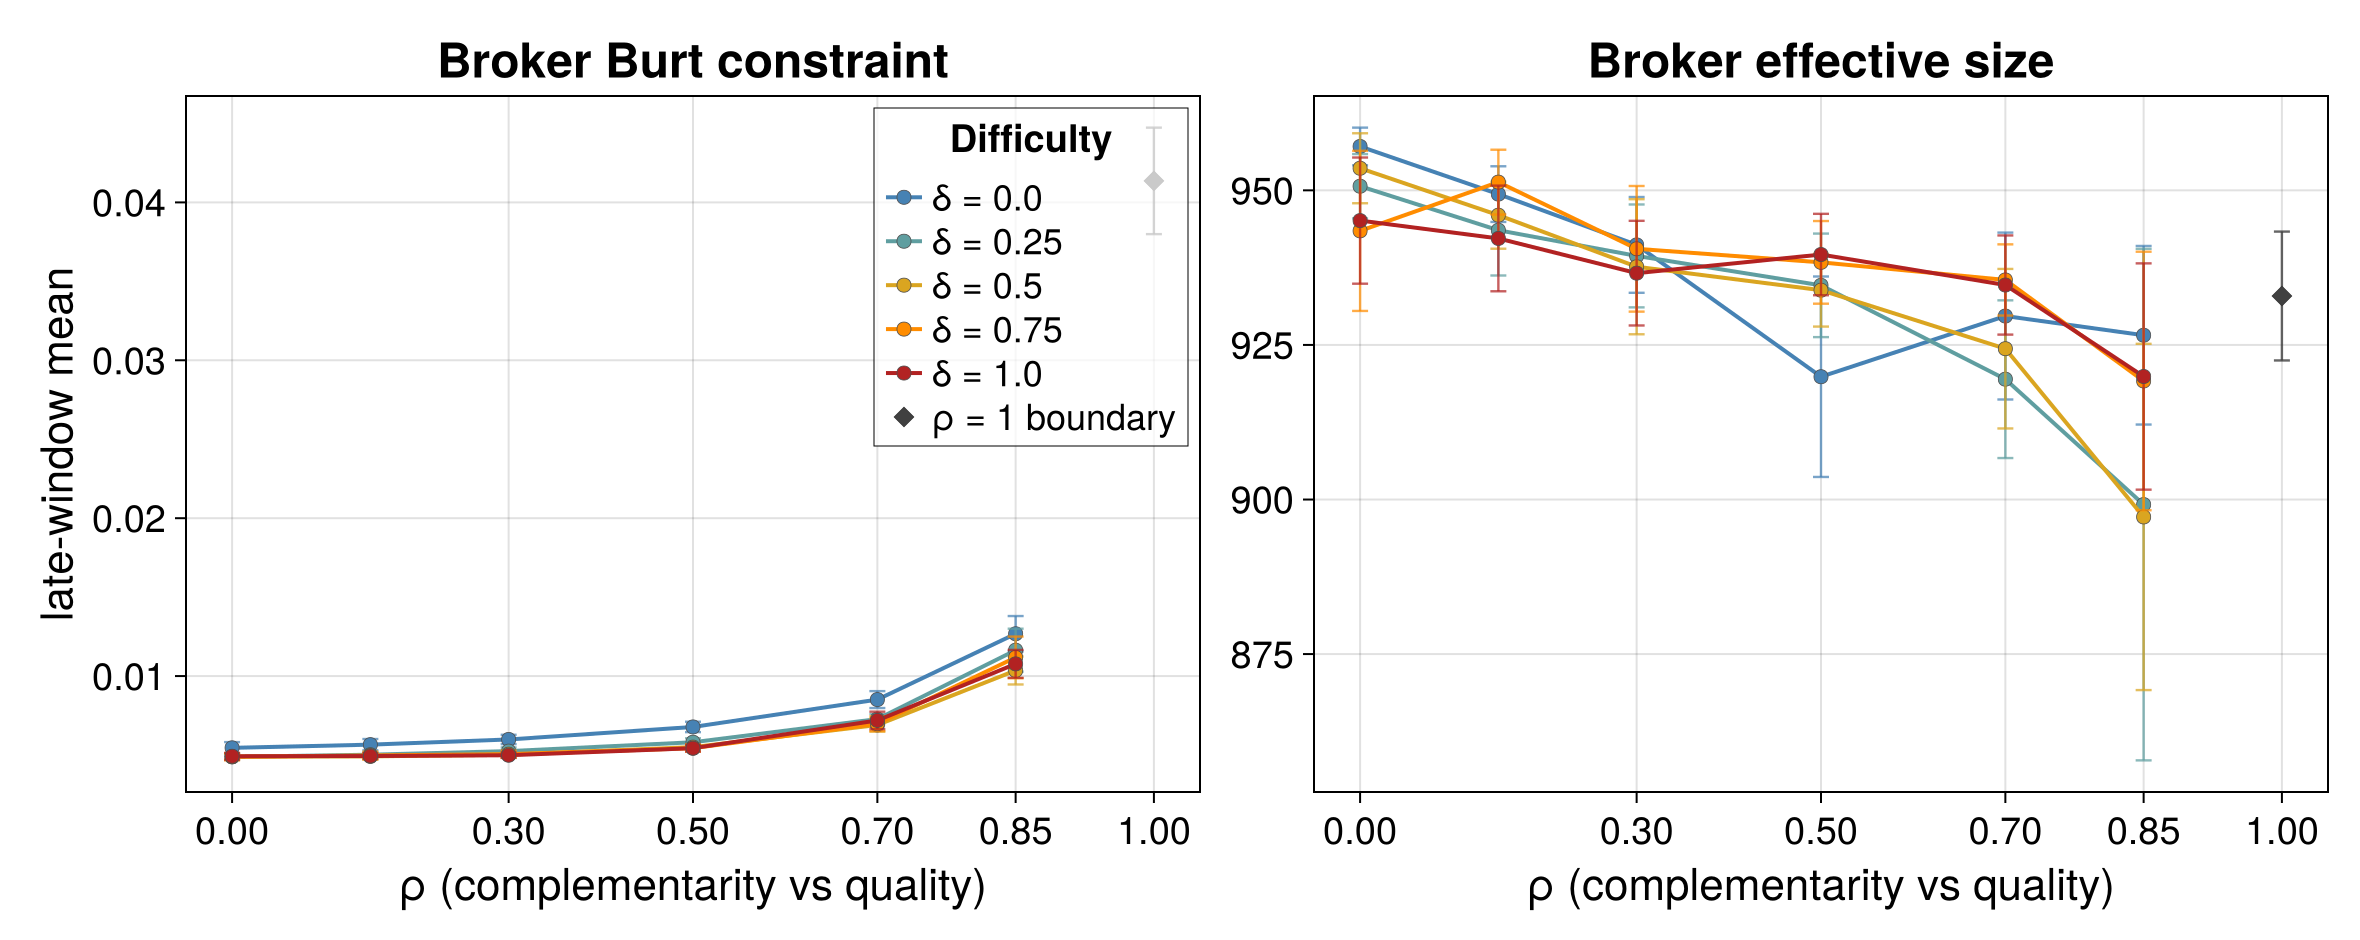
\includegraphics[width=\linewidth]{alternative_measures_grid.png}
\caption{\textbf{Alternative structural measures across the matching problem.} A: the broker's Burt constraint. B: the broker's effective size. General-quality share $\rho$ runs from pure complementarity (0) to pure general quality (1); colors and symbols identify difficulty $\delta$. Other parameters remain at baseline. The $\rho=1$ boundary, where difficulty is inactive, is shown once as an unconnected gray diamond. Points average periods 481--500 within each seed, then across seeds (\pv{suppBaselineSeeds} at baseline, \pv{suppOtherSeeds} otherwise). Whiskers are 95\% Monte Carlo intervals.}
\label{fig:supp-grid}
\end{figure}

\begin{figure}[htbp]
\centering
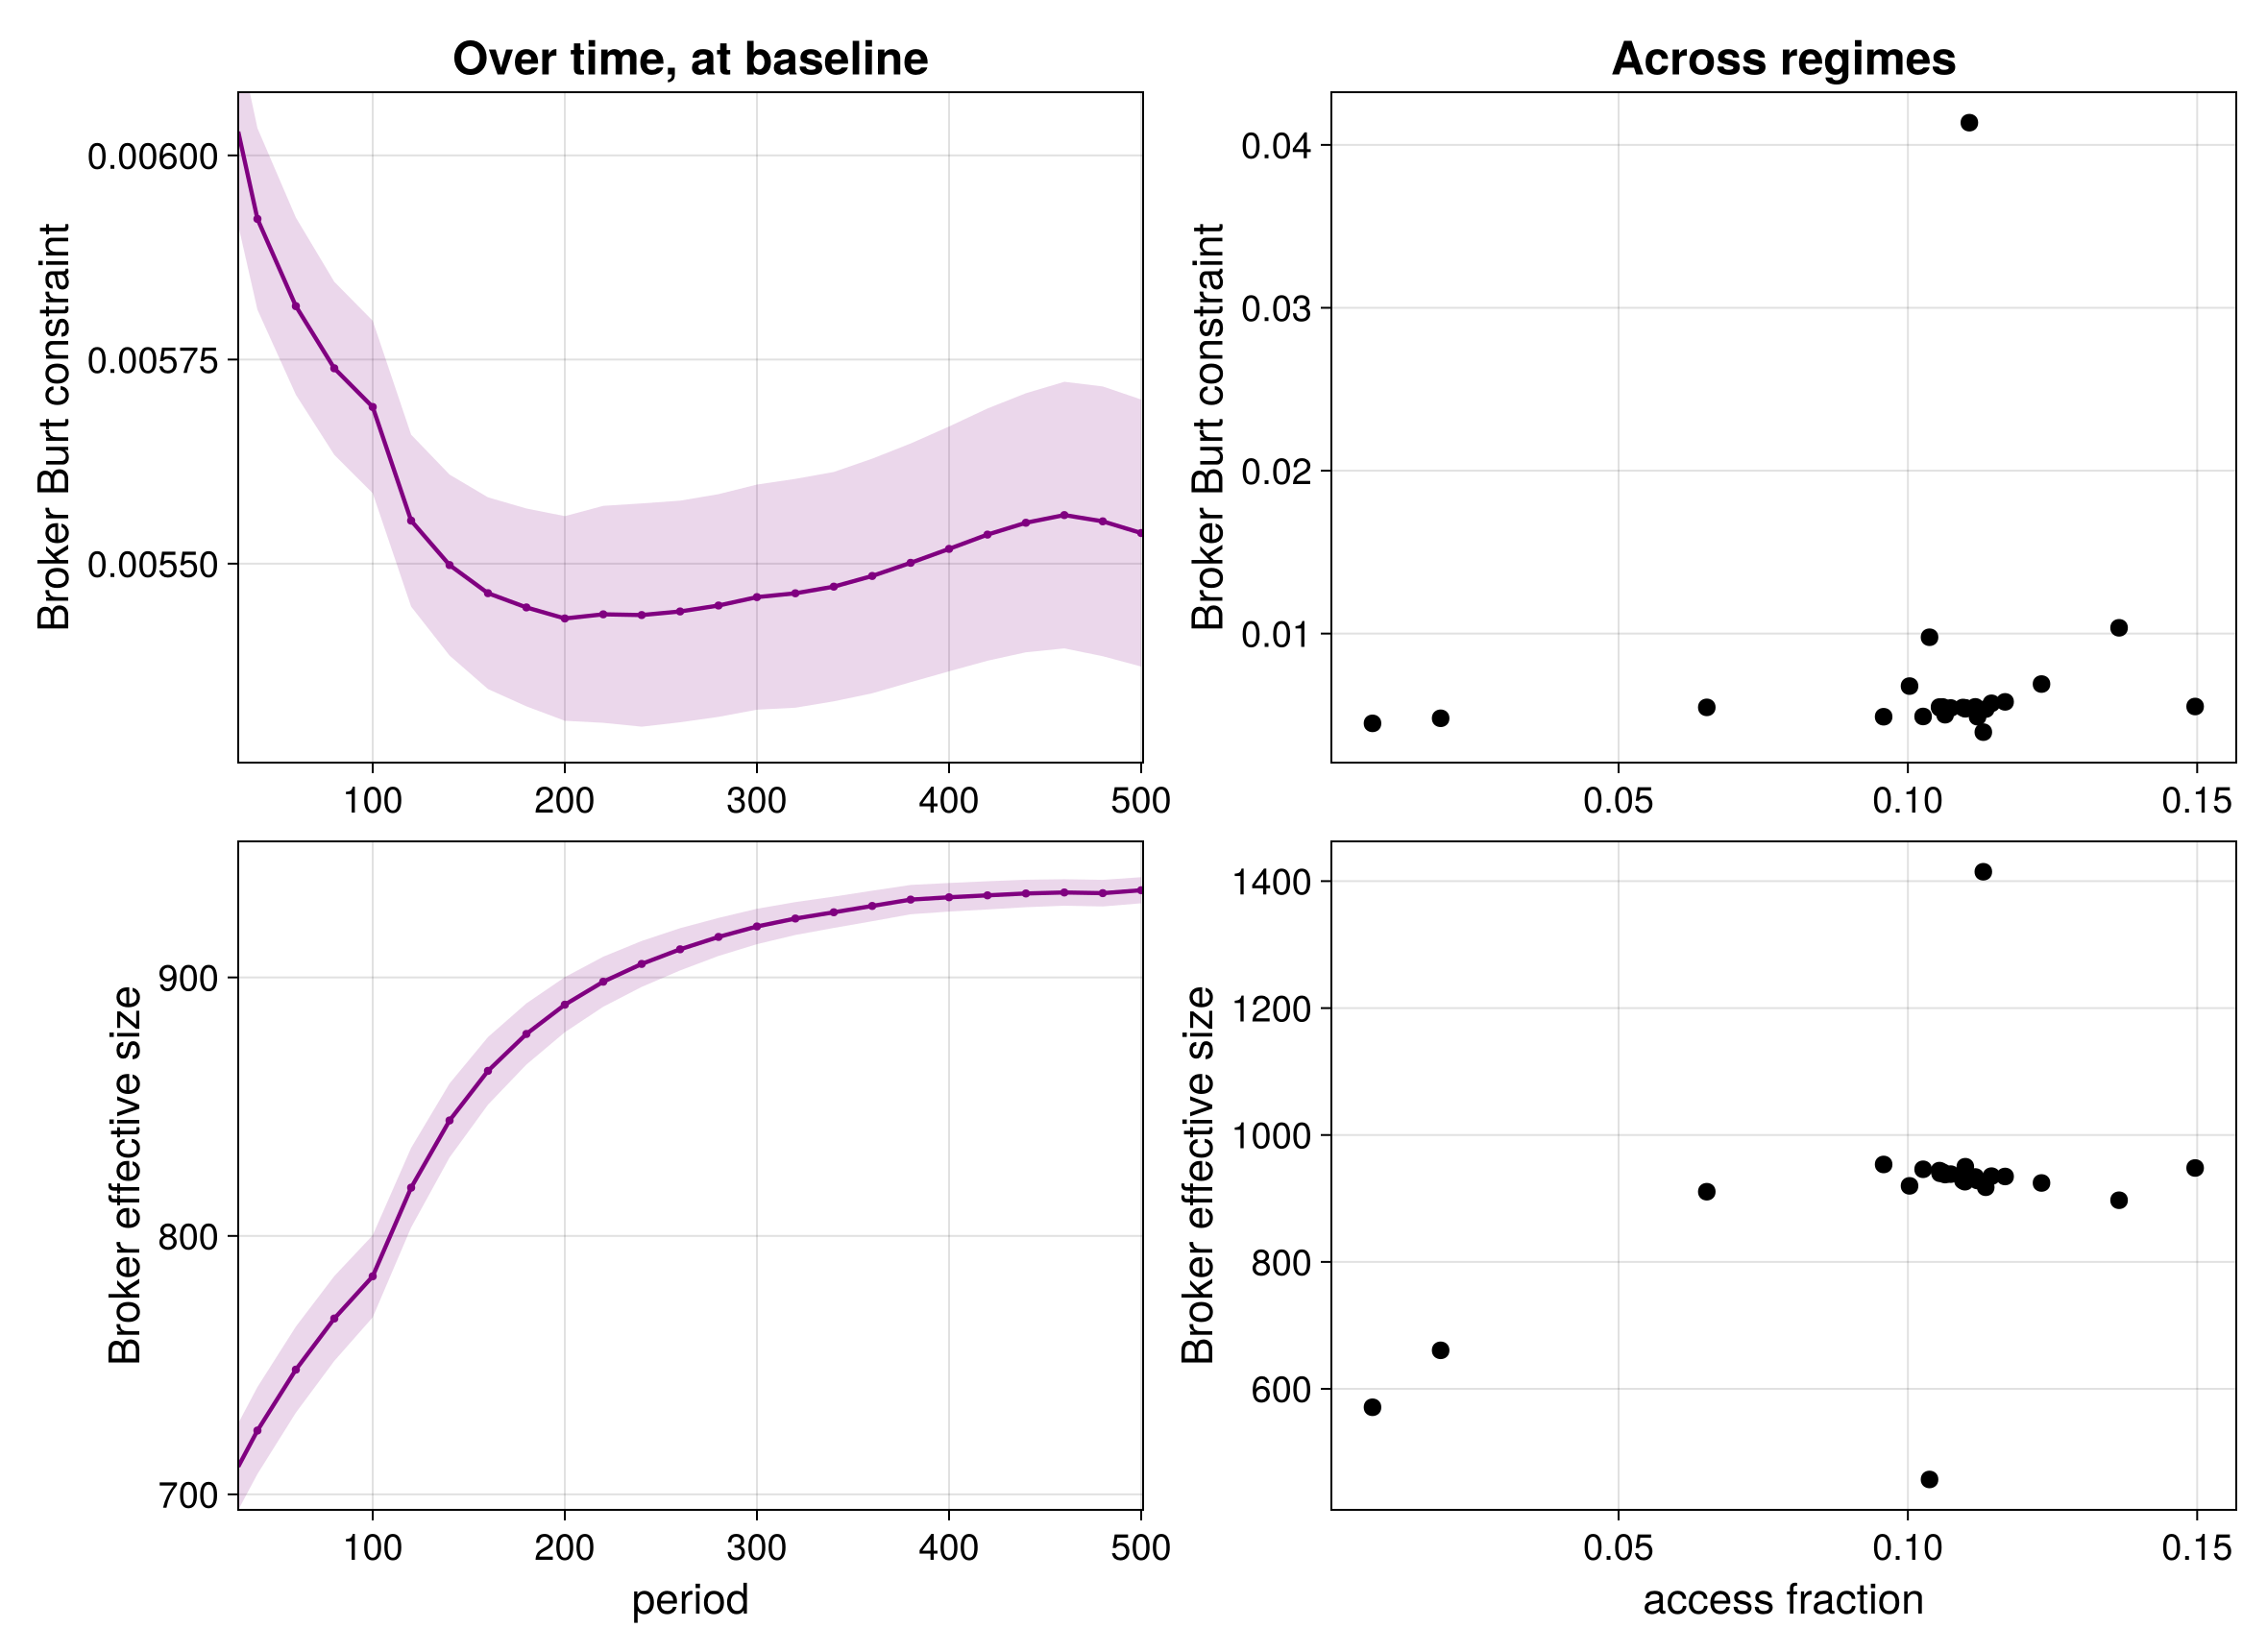
\includegraphics[width=\linewidth]{alternative_measures_position.png}
\caption{\textbf{Alternative structural measures over time and against access.} Top: the broker's Burt constraint. Bottom: the broker's effective size. A and C: baseline dynamics over \pv{suppBaselineSeeds} seeds. Measures are recorded every \pv{suppMeasInterval} periods and smoothed within each seed using a \pv{suppRollWin}-observation rolling mean. Lines are ensemble means; ribbons are pointwise 95\% Monte Carlo intervals. Time starts at $t=\pv{suppAxisStart}$ to omit initialization. B and D: the \pv{suppOatN} regimes that vary one parameter at a time from baseline. Points average periods 481--500 within each seed, then across seeds (\pv{suppBaselineSeeds} at baseline, \pv{suppOtherSeeds} otherwise). Access fraction is the share of brokered placements between principals with no pre-existing tie. Vertical scales differ between baseline dynamics and cross-regime comparisons.}
\label{fig:supp-position}
\end{figure}

\begin{figure}[htbp]
\centering
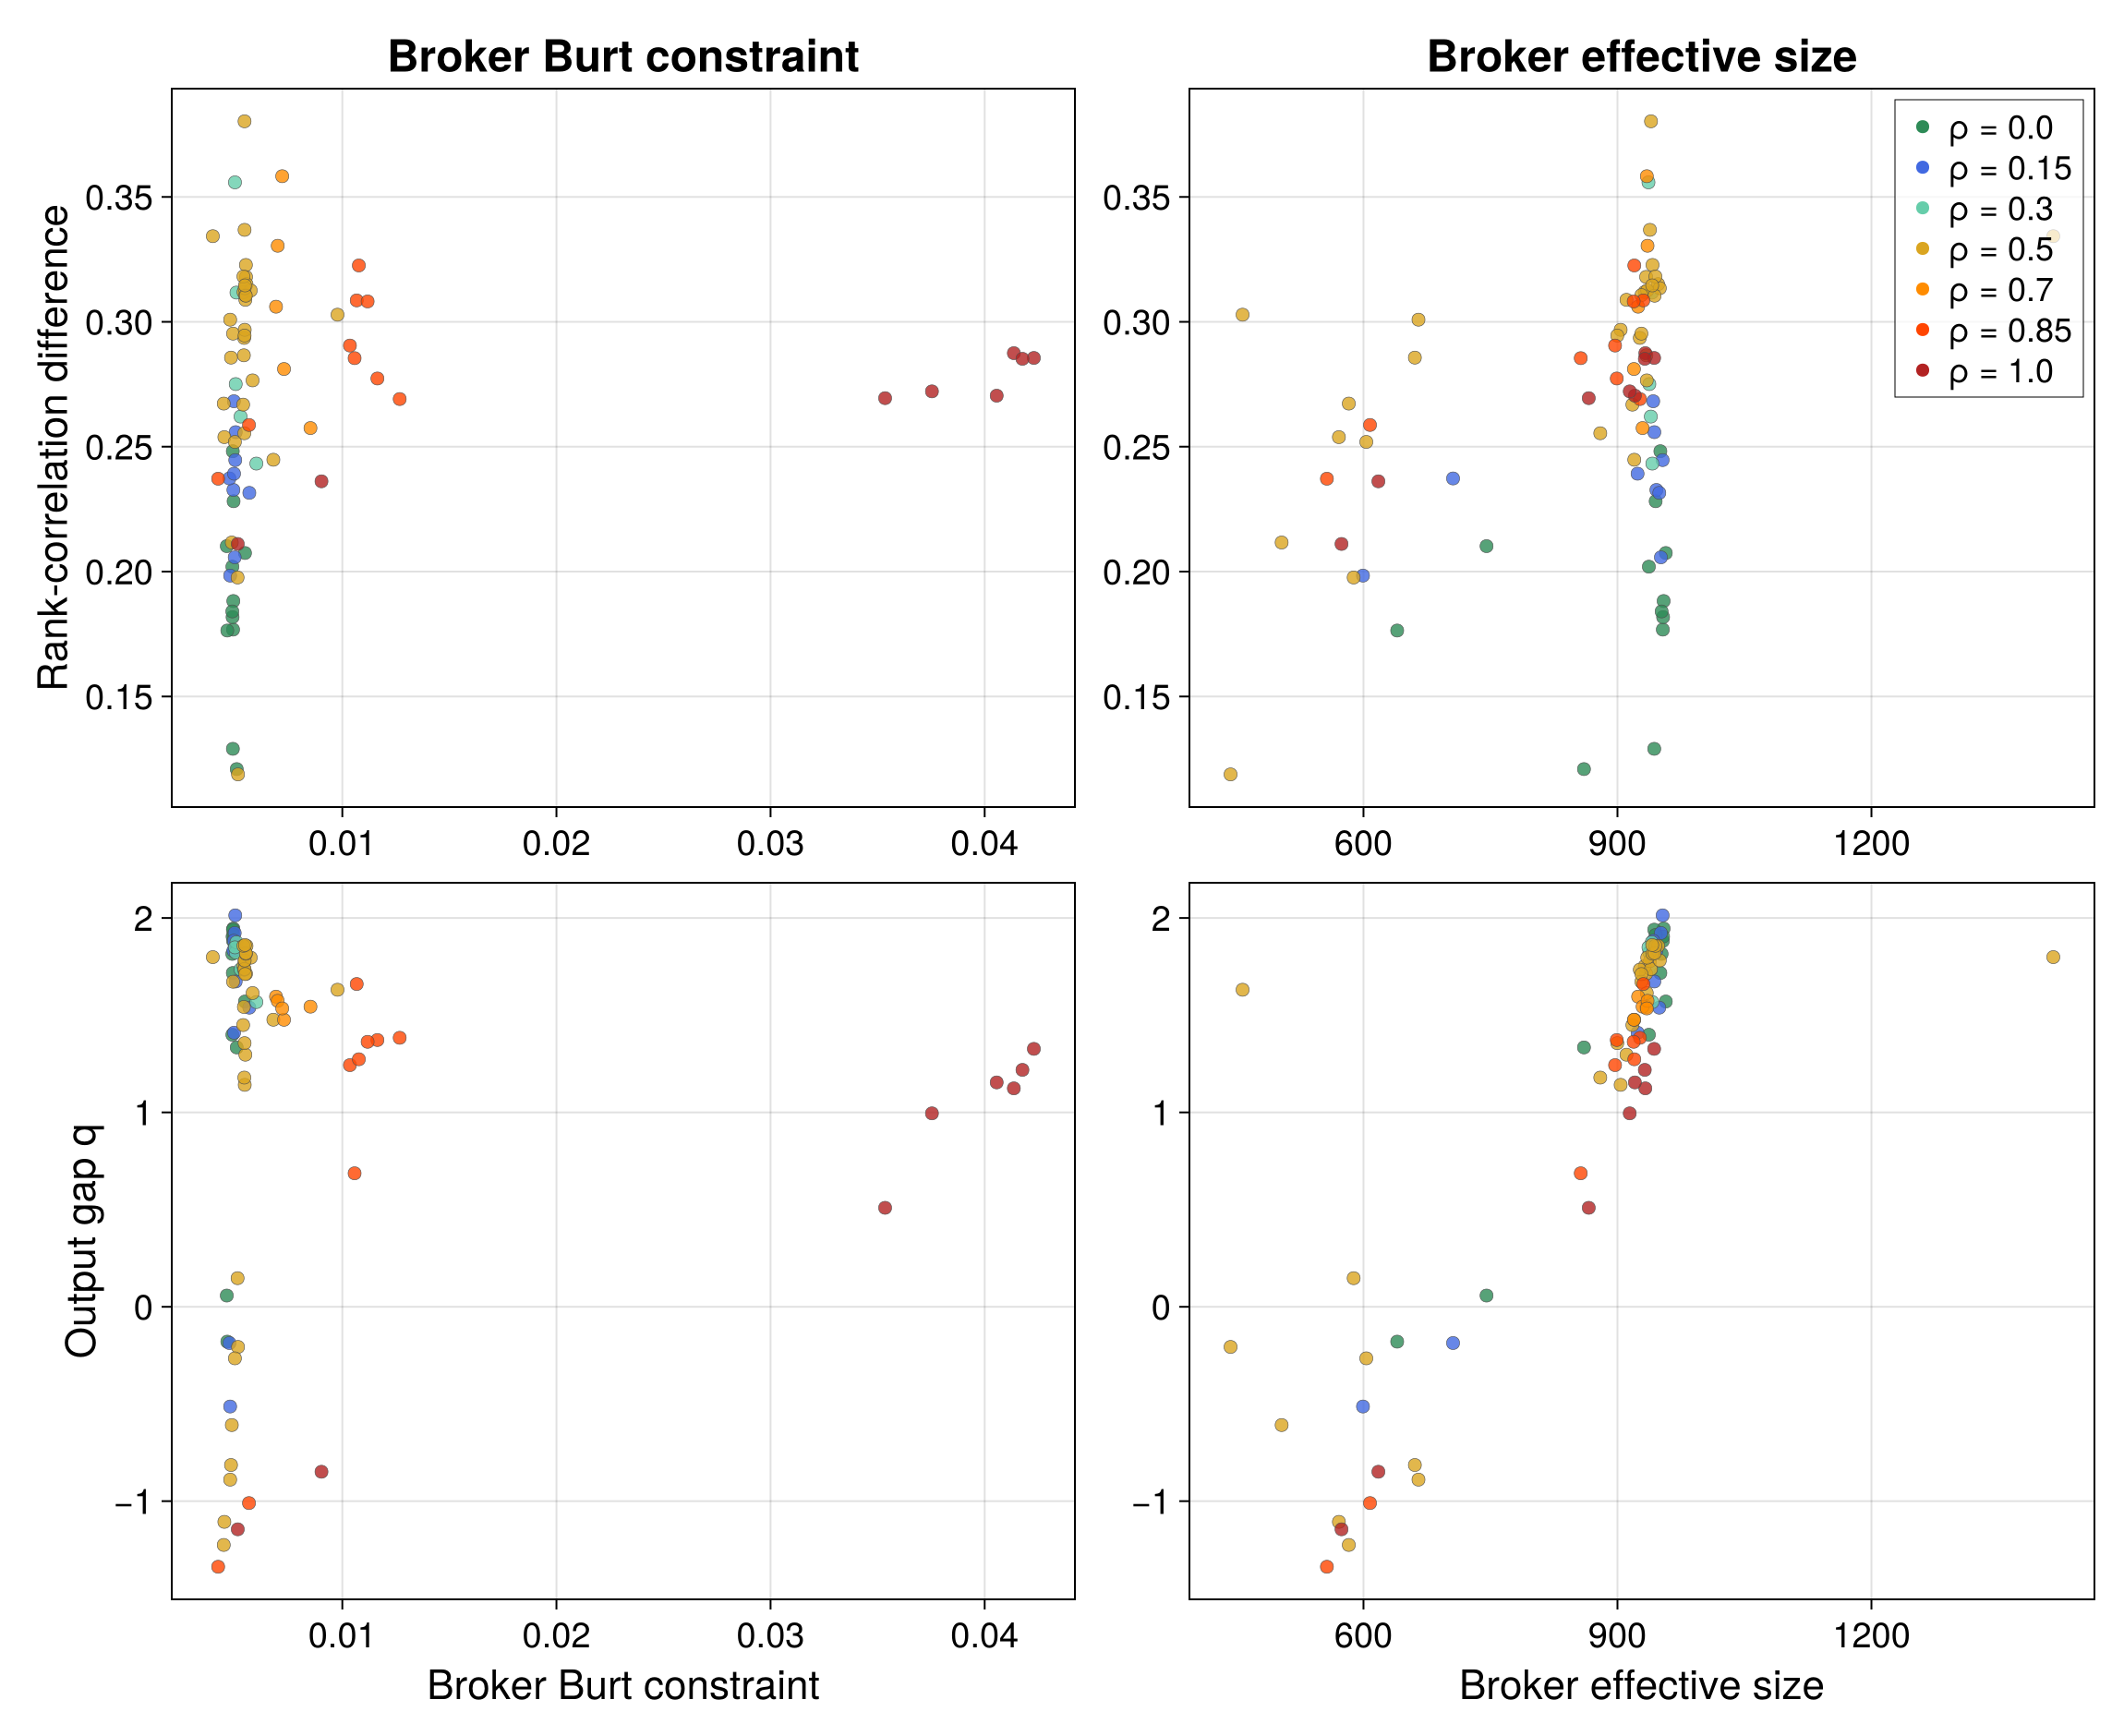
\includegraphics[width=\linewidth]{alternative_measures_advantage.png}
\caption{\textbf{Ranking and output differences by alternative structural measures.} A--B: difference in rank correlation between predicted and expected match output, broker minus principal. C--D: mean realized output per completed brokered match minus that per self-search match, before costs and fees. Horizontal axes show the broker's Burt constraint (A, C) or effective size (B, D). Each point represents one of the \pv{suppRegimeN} tested regimes, averaging periods 481--500 within each seed, then across seeds (\pv{suppBaselineSeeds} at baseline, \pv{suppOtherSeeds} otherwise). Colors and symbols identify general-quality share $\rho$, from pure complementarity (0) to pure general quality (1).}
\label{fig:supp-advantage}
\end{figure}

\end{document}
